%\documentclass{cumcmthesis}
\documentclass[withoutpreface,bwprint]{cumcmthesis} %去掉封面与编号页
%\usepackage{graphicx}
%\usepackage{subfigure}
\usepackage{tabularx}
\usepackage{yhmath}
\title{论文题目}
\tihao{B}            % 题号
\baominghao{202217241200}    % 报名号
\schoolname{华中科技大学}
\membera{卢凯}
\memberb{陈铭锐}
\memberc{房怿宽}
\supervisor{胡勇}
\yearinput{2022}     % 年
\monthinput{09}      % 月
\dayinput{15}        % 日
\usepackage{algpseudocode}
\usepackage{amsmath}
\makeatletter
\newif\if@restonecol
\makeatother
\let\algorithm\relax
\let\endalgorithm\relax
\usepackage[linesnumbered,ruled,vlined]{algorithm2e}%[ruled,vlined]{
\DeclareSymbolFont{yhlargesymbols}{OMX}{yhex}{m}{n}
\DeclareSymbolFont{ugmL}{OMX}{mdugm}{m}{n}
\DeclareMathAccent{\wideparen}{\mathord}{yhlargesymbols}{"F3}
\renewcommand{\algorithmicrequire}{\textbf{Input:}}  % Use Input in the format of Algorithm
\renewcommand{\algorithmicensure}{\textbf{Output:}} % Use Output in the format of Algorithm
\begin{document}
	\maketitle
	\begin{abstract}
		摘要的具体内容。
		\keywords{关键词1\quad  关键词2\quad   关键词3}
	\end{abstract}
	%\tableofcontents
	
	
%----------- 正文 ----------
%----------- 一、问题重述 ----------
		\section{问题重述}
		\subsection{问题背景}
		\par 无人机是“无人驾驶空中飞行器”(UAV)的简称。1917年首先由英国研制出来最先承担起军事功能,诸如目标定位跟踪技术在航空、航天和航海领域都有十分重要的地位。无源定位技术是被动工作方式的目标定位技术,利用未知目标的辐射源信号进行定位和导航。
		\subsection{待求解的问题}
		\par 
		\begin{enumerate}
			\item{\textbf{问题一(1)}:}在已知三架编号已知、位置无偏差的无人机且其中一架为位于圆心的无人机FY$ 00 $为承担发射信号任务的无人机的既定条件下,根据圆周上其他的位置存在偏差的无人机被动接受的方向信号建立模型来完成对该被动接收信号无人机的纯方位无源定位。
			\item{\textbf{问题一(2)}:}在编队方式仍为圆周,且无人机数目仍为10架的相同条件下,修改发射信号的无人机为编号FY$ 00 $和FY$ 01 $的无人机与待定数量未知编号的无人机。发射信号的无人机的位置没有偏差,确定除了已知编号的无人机FY$ 00 $和无人机FY$ 01 $外,最少需要几架未知编号的无人机作为位置无偏差的无人机来发射信号以期望实现无人机的有效定位。
			\item{\textbf{问题一(3)}:}在编队方式与无人机数目基础条件均不变的基础上,设定无人机所处圆周的半径为100m。初始时刻无人机的位置确定但略有偏差,试确定在编号为FY$ 00 $的无人机和圆周上数量不超过三架的无人机作为发射信号的无人机的条件下,忽略每次调整的时间,调整到理想位置使九架无人机均匀的分布在某个圆周上的最优调整方案。
			\item{\textbf{问题二}:}
		\end{enumerate}
%----------- 二、问题分析 ----------
	\section{问题分析}
		\subsection{问题一(1):}
		在第一题的大背景下,我们可以知道,无人机的数目和编队的方式,并且给定的条件为有三架已知编号且位置没有误差的无人机作为发射信号的无人机。我们需要根据其余位置有偏差的无人机被动接受到的方位信号即三个角度信息从而实现定位。
		\subsection{问题一(2):}
		在问题一(2)中,我们首先假设对于任意的$D_i$,通过测量$D_0,D_1,D_j$三个无人机的位置,得到两个小角$\alpha_1,\alpha_2$,进而能够确定自己在$D_0 - D_1$坐标系中的位置。
		
		可以假定的是,对于任意的$D_i$,在接收其他无人机的发射信号时,有以下公共知识:
		\begin{itemize}
			\item	位置待定无人机自身的编号$i$,
			\item	可以辨识从$D_0$与$D_1$发出的信号,但不确定第三个信号来源,
			\item	无人机机群的结构,即各个编号无人机在圆上的大致位置与顺序,任意两个无人机不能交换顺序,
			\item 	待定无人机相对于理想位置的偏差较小,即$ {\lVert \omega_i \rVert}^2 < r_0 $.
		\end{itemize}
		\begin{figure}[htb]
			\centering
			\subfloat[组态1]{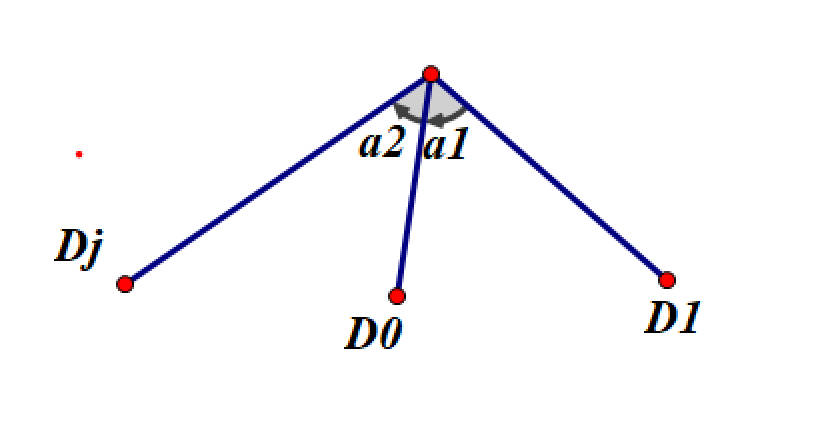
\includegraphics[width=0.4\linewidth]{../figures/1}}
			\subfloat[组态2]{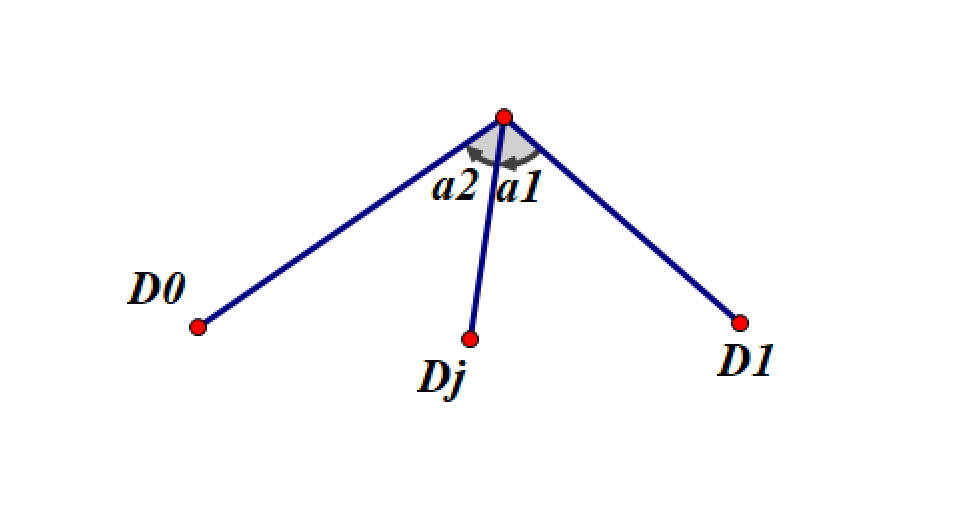
\includegraphics[width=0.4\linewidth]{../figures/2}}
			\caption{可能出现的两种组态}
			\label{fig1}
		\end{figure}
		基于以上公共知识,需要设计算法$D_i = f(\alpha_1, \alpha_2)$求解$D_i$在$D_0 - D_1$坐标系中的位置。
		\subsection{问题一(3):}
		在问题三中,我们认为9架飞机均匀分布在以编号FY00为圆心的情况为理想分布,要求在各无人机所在位置与理想位置略有偏差的初始情况下,每次通过选取FY00和圆上最多三架飞机发射信号,其余飞机根据接收到的方向信息调整位置。我们得到如下分析和和假设:
		\begin{itemize}
			\item	每个飞机知道自身的编号$i$和自身的理想分布位置$(x_{ideal},y_{ideal})$
			\item   飞机对每个接收到的信号,能够识别其信号来源无人机的编号$i$,
			\item	每个飞机根据接收到的方向信息进行定位,得到估计定位$(\hat{x},\hat{y})$,通过位移一段距离进行调整位置调整,位移在直角坐标系下表示为$(\Delta{}x,\Delta{}y)$,可以度量估计定位$(\hat{x},\hat{y})$和理想位置$(x_ideal,y_ideal)$的偏差来确定,
			\item	由于发射信号的飞机可能有误差,所以使用基于问题一的定位方法会产生误差,
			\item 	待定无人机相对于理想位置的偏差较小,即$ {\lVert \omega_i \rVert}^2 < r_0 $.
		\end{itemize}
		基于上述分析,我们建立了一个位置调整算法,对输入的起始情况,对编号为$i$的飞机,通过多次迭代$(\Delta{}x,\Delta{}y)_i$调整位置,将机群调整到理想分布上。该算法可以分为选取发射信号飞机、接收信号与定位、位置调整三个部分。
		\subsection{问题二:}
%----------- 三、模型的假设与约定 ----------
	\section{模型的假设与约定}
		\begin{itemize}
			\item{} one
			\item{} two
			\item{} three
		\end{itemize}
%----------- 四、符号说明及名词定义 ----------
	\section{符号说明及名词定义}
		\begin{center}
			\begin{table}[H]
				\caption{本论文所使用的符号}
				\begin{tabularx}{\textwidth}{p{0.08\textwidth}X}
					\toprule	
					$D_i$ & 编号为$i$的无人机的理想位置  \\
					$\widehat{D_i}$ & 编号为$i$的无人机的有偏实际位置  \\
					$D_i(\rho,\theta)$ & 用极坐标表示的无人机的位置 \\
					  
					$\overrightarrow{D_iD_k}$ & 从$D_i$指向$D_k$的矢量 \\
					$\omega_i$      & 编号为$i$的无人机的误差矢量,即$\overrightarrow{\widehat{D_i}D_i}$ \\
					$\bigodot O_i$    & 第$i$个理想圆  \\
					\bottomrule
				\end{tabularx}
			\end{table}

		\end{center}
%----------- 五、模型的建立与求解 ----------
	\section{模型的建立与求解}
		\subsection{问题一(1)}
			\subsubsection{问题一(1)模型的建立}
			\par 问题一首先限定了编队的飞机数目为10架并且编队方式为圆形编队,且要求其中一架无人机(编号为FY$ 00 $)位于圆心,而其余九架无人机位于相应的圆周上面。值得注意的是,无人机会基于自身感知的高度信息,均保持在同一个高度上飞行,因此我们可以将问题的求解模型确定在一个高度平面来方便求解下列各个问题。
			\par 
			而第一题的第一问则进一步明确无人机的角色:位于圆心的无人机(FY$ 00 $)和编队中另 $ 2 $ 架无人机发射信号,而其他无人机则是被动接受该三架无人机发射信号的角色。同时一个重要的条件是:模型要求在发射信号的无人机位置无偏差且编号已知的情况下完成其他被动接受信号的无人的定位。基于上述已知设定信息,我们可以首先将定位问题转换为二维平面上的位置求解问题。因为圆周的位置具有\textbf{高度对称性},因此不妨假设其中两台圆周上已知编号的信号发射无人机其中一台的编号为FY$ 01 $.因此我们可以在二维平面上选取编号为FY$ 00 $的无人机为原点,编号为FY$ 01 $的无人机为$ X $轴正方向的一点,从而建立笛卡尔右手坐标系如下图\ref{1-1}。
			\begin{figure}[htb]
				\centering
				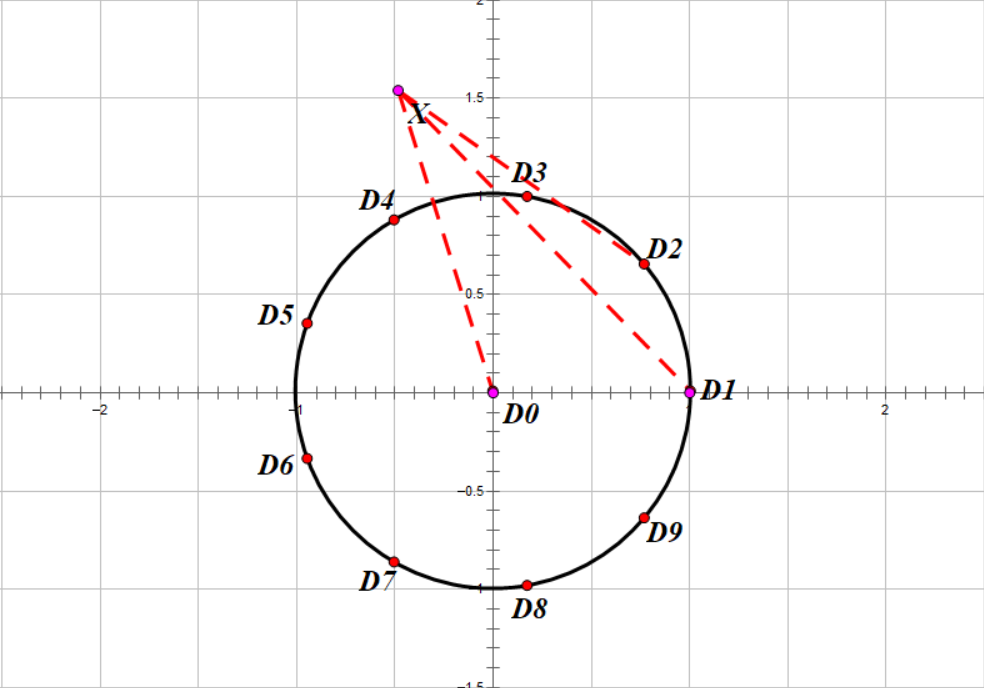
\includegraphics[width=0.7\linewidth]{./figures/Question1-1.png}
				\caption{问题一:定位模型坐标系}
				\label{1-1}
			\end{figure}
			在已知三架编号已知且位置无偏差的无人机后,我们可以在该坐标系中按直角坐标。同时对于编队中其他待定位的无人机,我们都可以得到与三架发射信号无人机的方位信息:任意两架发射信号无人机与待定位无人机的夹角。夹角代表着方向向量直接的位置关系,故应在表示待定位无人机的直角坐标后确定发射信号的无人机与待定位无人机连线的方向向量,进而再表示出夹角然后求解。
			\subsubsection{问题一(1)的具体求解}
			\par 基于第一问的定位模型,我们建立以已知编号FY$ 00 $ 的无人机为原点$ D_0 $ ,而另外两架已知编号的$ \text{无人机}i\text{与无人机}j $ $ \text{无人机}i\text{与无人机}j $ 分别设为$ D_i\text{与}D_j $ ,其极坐标对应的为$ \left( R,\beta _i \right) ,\left( R,\beta _j \right)  $ ,其中$ \beta _i\text{与}\beta _j $ 均可通过编号得到,为已知数据。不失一般性,我们将其他所有待定位的无人机$ D_X $ 的极坐标设为$ \left( \rho ,\theta \right)  $ 。根据题意我们可知无人机$  D_X $ 会接收到位于设定原点的无人机$ D_0 $ 和$ \text{无人机}D_i\text{与无人机}D_j $ 发射的电磁信号,进而可以提取的信号为:该无人机$ D_X $ 与任意两架发射信号的$ \text{无人机}D_i\text{与无人机}D_j $ 连线之间的夹角,即$ \left( \begin{array}{c} 	3\\ 	2\\ \end{array} \right)  $ 共三个角度的方位信息。根据几何知识,可以得到该三个角中最大的角为其余两个角的和。因此,为减少信息的冗余性,我们只利用其中两个角:$$ \alpha _i=\angle D_0 D_X D_i\text{,}\alpha _j=\angle D_0 D_X D_j $$ 
			\par 至此,我们从极坐标转至直角坐标系: 
			$$ D_0\text{:}\left( 0,0 \right)  $$ $$ D_i\text{:}\left( R\cos \beta _i,R\sin \beta _i \right)  $$ $$ D_j\text{:}\left( R\cos \beta _j,R\sin \beta _j \right)  $$ $$ D_X\text{:}\left( \rho \cos \theta ,\rho \sin \theta \right)  $$ 
			\par 因此可以进而得到三个向量:
			$$ \overrightarrow{D_0D_X}=\left( \rho \cos \theta ,\rho \sin \theta \right)  $$ $$ \overrightarrow{D_iD_X}=\left( \rho \cos \theta -r\cos \beta _i,\rho \sin \theta -R\sin \beta _i \right)  $$ $$ \overrightarrow{D_jD_X}=\left( \rho \cos \theta -R\cos \beta _j,\rho \sin \theta -R\sin \beta _j \right)  $$ 	
			\par 紧接着,我们通过三个向量分别利用余弦定理,分别表示出$ \alpha _i\text{与}\alpha _j $: 
			$$ \cos \alpha _k=\frac{\rho ^2\sin ^2\theta -R\rho \cos \beta _k\cos \theta +\rho ^2\cos ^2\theta -R\rho \sin \beta _k\sin \theta}{\rho ·\sqrt{\rho ^2\sin ^2\theta +r^2\sin ^2\beta _k-2R\rho \sin \beta _k\sin \theta +\rho ^2\cos ^2\theta +R^2\cos ^2\beta _k-2R\rho \cos \beta _k\cos \theta}}\\   $$ 
			
			$$\text{令} k=i,j\text{可分别得}\left\{ \begin{array}{l} 	\cos \alpha _i=\frac{\rho -R\cos \left( \theta -\beta _i \right)}{\sqrt{\rho ^2+R^2-2\rho R\cos \left( \theta -\beta _i \right)}}\\ 	\cos \alpha _j=\frac{\rho -R\cos \left( \theta -\beta _j \right)}{\sqrt{\rho ^2+R^2-2\rho R\cos \left( \theta -\beta _j \right)}} \end{array} \right.  $$ 
			\par 由此求解 两个方程:$ \text{通过}\frac{\rho}{R}\text{和}\theta \text{表示的}D_X\text{具体坐标} $ 从而完成定位。
			
		\subsection{问题一(2)}
			经过我们的研究,我们认为需要除了在圆心的0号,还需要在圆弧上的1号和另外一个j号共三架飞机发射信号才能确定任意一架飞机i的位置。
			我们的位置解算算法遵循机组组态分析、推断匿名第三者编号、可行域分割的步骤求出$D_i$的坐标。在使用逐步分割可行域的方式求解位置坐标时,我们针对多解的情况,着重讨论了对于“略有偏差”的数学定义。
			\subsubsection{算法的求解过程分析}
			对于问题$D_i = f(\alpha_1, \alpha_2)$,因为第一问中我们已经求解出了对于确定圆周上两个信号发射飞机的编号时,待测飞机位置的解析算法。本问我们首先需要确定第三架飞机是标签为几的飞机。以待测飞机为2号机,匿名第三信号发射机为3号机为例,建立数学几何模型并阐释我们的算法。
			\paragraph{机组组态分析}
			待测飞机为2号机的情况下,2号机接收到的三个角度值遵循$\angle D_jD_2D_1 =\angle D_jD_2D_0 + \angle D_jD_2D_1$,符合图\ref{fig1}中所示组态1的类型。
			\paragraph{匿名第三者位置分析}
			在组态1的情况下,匿名第三者编号$j=3,4,5,6$中的一个。
			\paragraph{可行域}
			对于所有可能的$D_j$,现已确定$\angle D_jD_2D_0 = \alpha_1$,$|D_jD_0|= r$,对于此类定弦定角问题,有优弧$\wideparen{D_jD_2D_0}$上的点为所有可能的$D_2$的位置。
			对于确定的$\angle D_0D_2D_1 = \alpha_2$,$|D_1D_0|= r$优弧$\wideparen{D_0D_2D_1}$上的所有点为所有可能的的$D_2$的位置。
			\begin{figure}[htb]
				\centering
				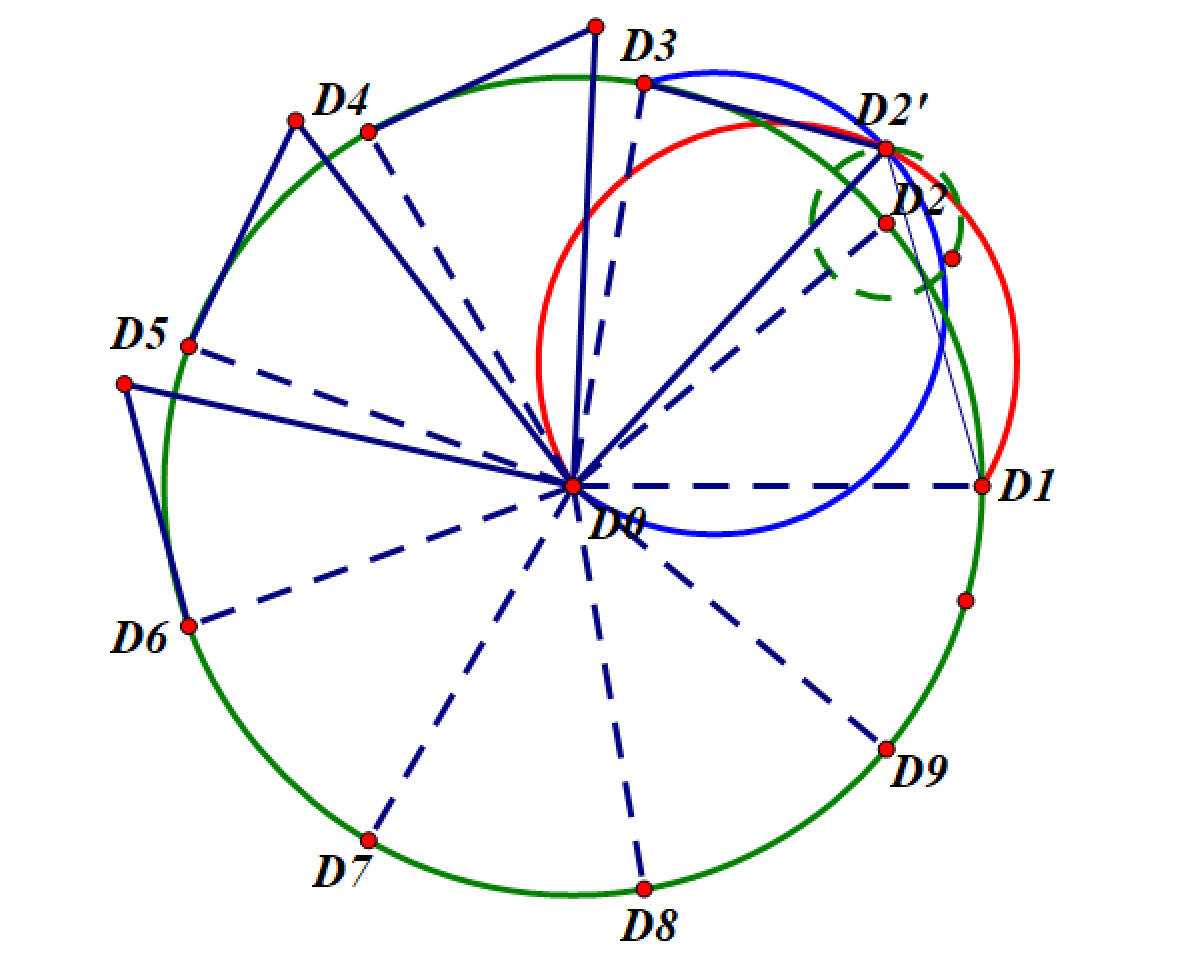
\includegraphics[width=0.5\linewidth]{./figures/3}
				\caption{$\angle D_3D_2D_0$ 的可行域$\wideparen{D_3D_2D_0}$与$\angle D_0D_2D_1$ 的可行域$\wideparen{D_0D_2D_1}$}
				\label{fig3}
			\end{figure}
		
		
			如图\ref{fig3}所示,对于有微小偏差的无人机$D_2'$,当假设匿名第三者为无人机3时,有可能位置$P$。同理,分别建立匿名第三者$j=4,5,6$时,$D_2'$的可能位置,分别标记为$Q,R,S$,如图\ref{fig4}.
			
			\begin{figure}[htb]
				\centering
				\subfloat[所有可能可行域集合]{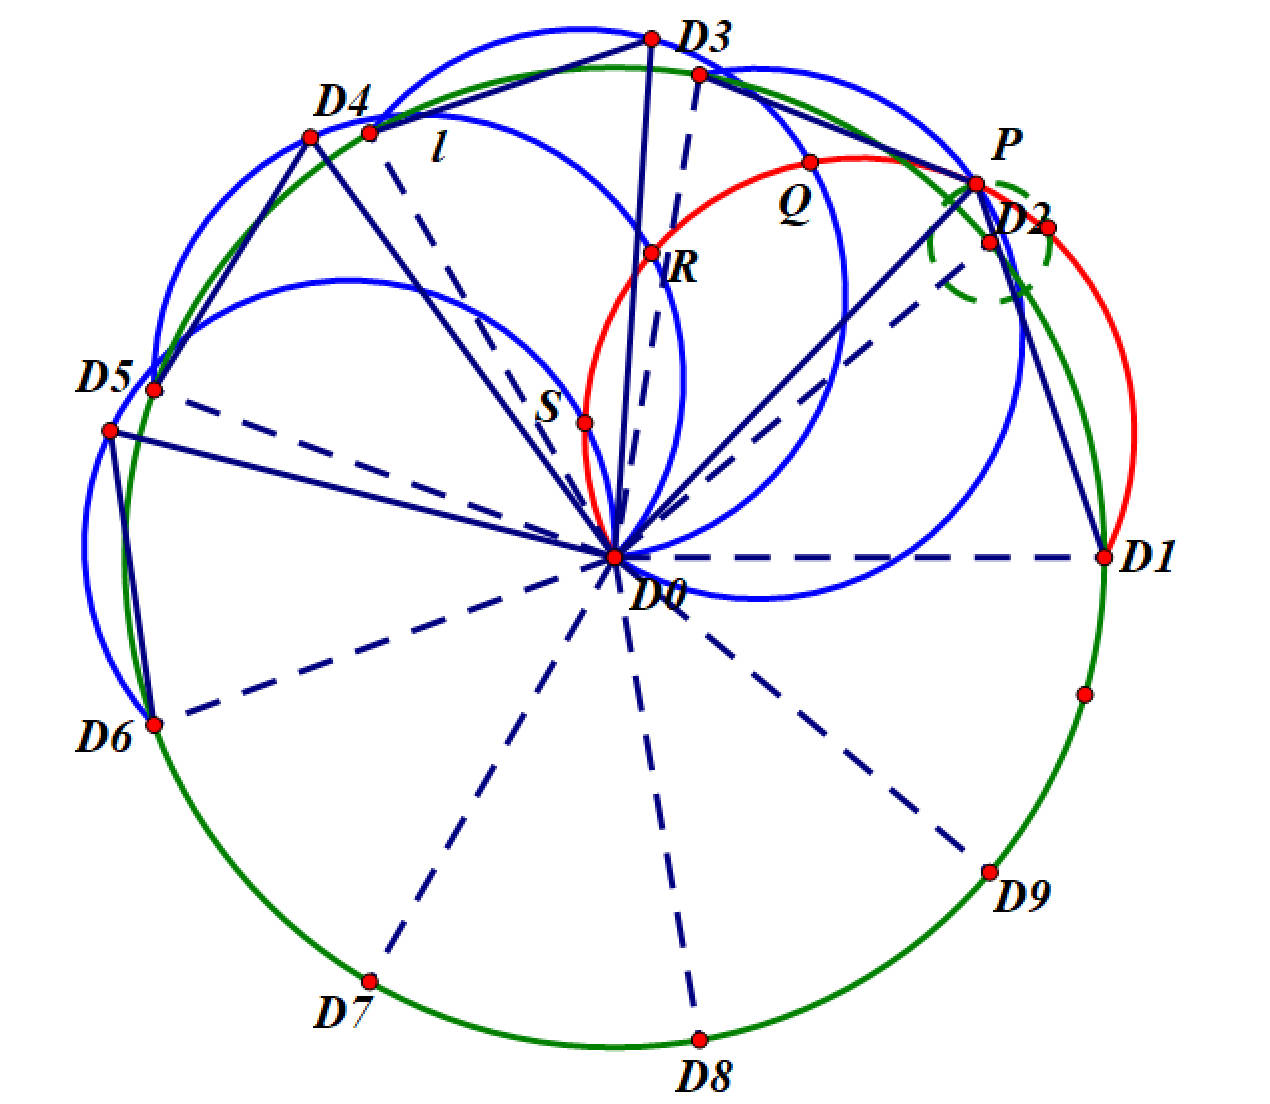
\includegraphics[width=0.4\linewidth]{../figures/4}}
				\subfloat[$D_2'$的可能位置$P,Q,R$]{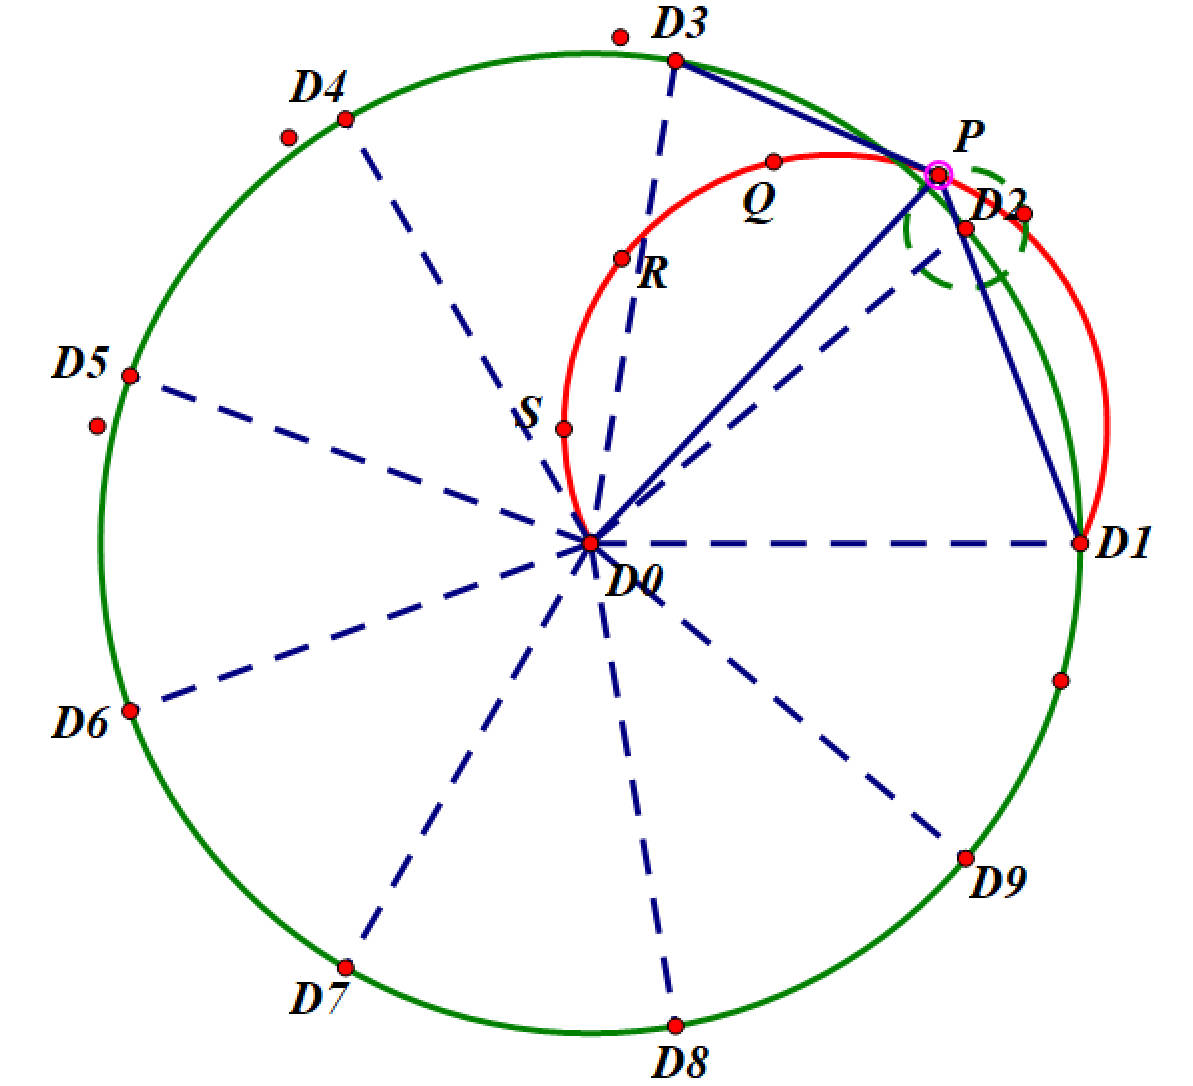
\includegraphics[width=0.4\linewidth]{../figures/5}}
				\caption{$D_2'$的可能位置的求解}
				\label{fig4}
			\end{figure}
			
			至此,对于不确定匿名第三者的情形,飞机$D_i$($D_2$)由于不能确定第三者编号产生了自己的位置猜测$P,Q,R,S$,在图\ref{fig4}的情形下,易确定$R,S$的情形不符合题设从而排除,然而我们观察到当2号机偏差很大时(即$\lVert\omega_i\rVert =\overrightarrow{D_2D_2'} $很大时)有可能出现情形如图\ref{fig6}.此时若认为第三者为4号机,则会有位置错误估计Q,而不是其实际位置P。因为此种情况的存在,我们就不能单纯地使用推断点距离理想点最近的一点作为测量结果,而要对“偏差较小”进行数学定义。
			\begin{figure}[htb]
				\centering
				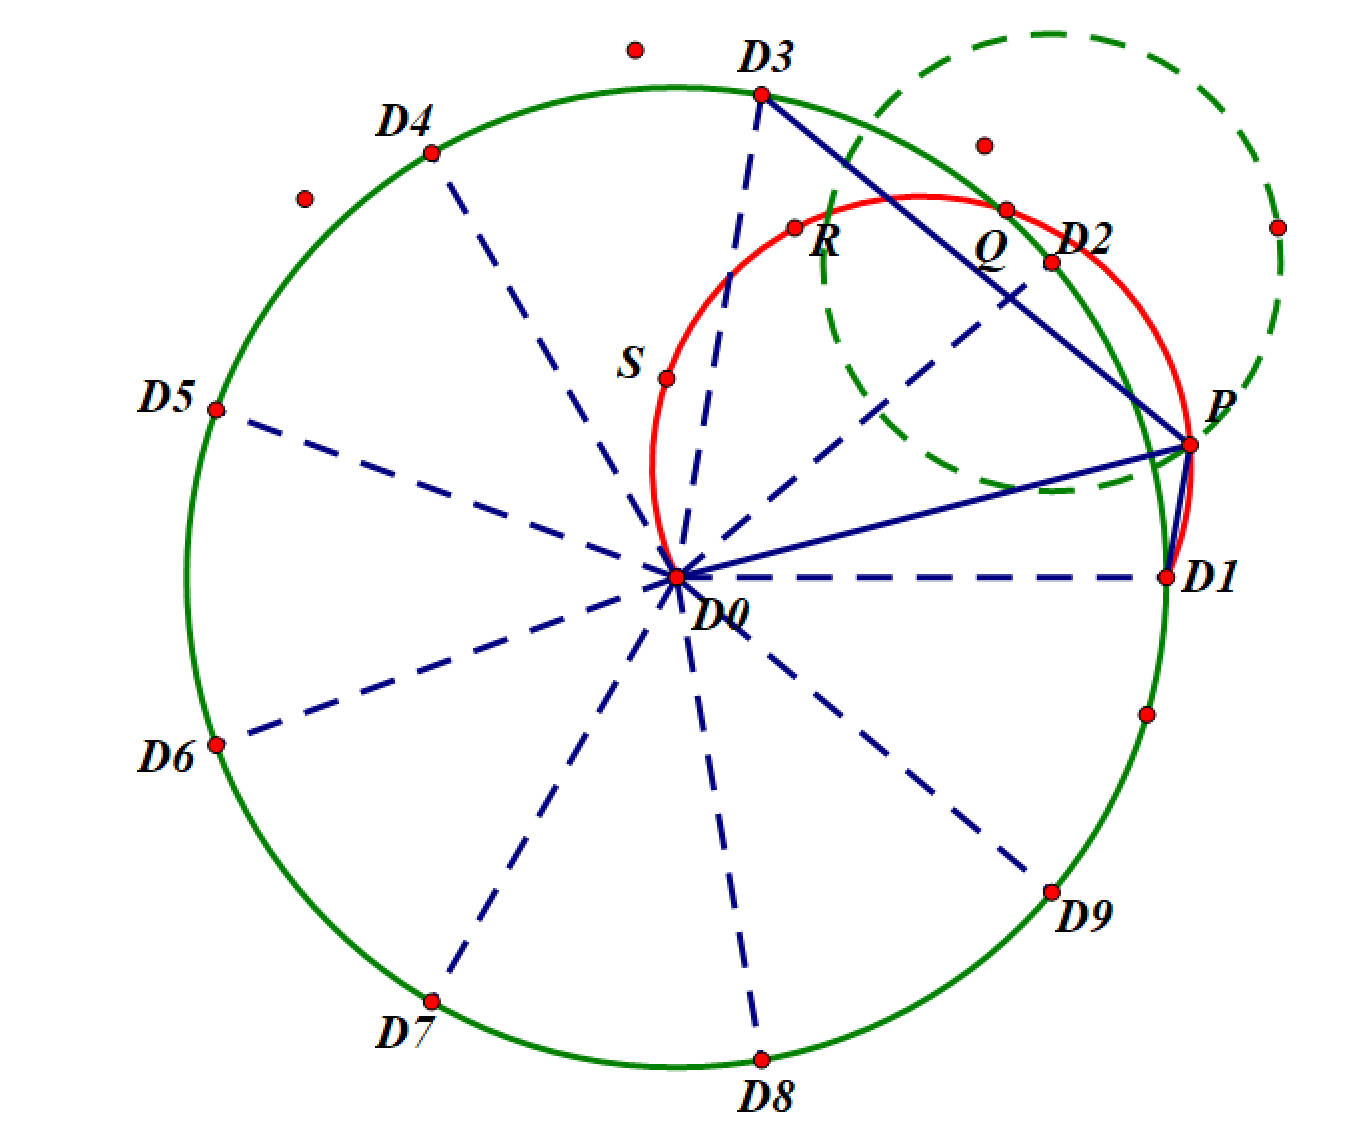
\includegraphics[width=0.5\linewidth]{./figures/6}
				\caption{偏差很大时的一种特殊情况}
				\label{fig6}
			\end{figure}
		
		
			\paragraph{多解分析}
			因为在三架飞机定位的模式下,匿名第三者未知。这种情况下待定位飞机对于自己的位置估计就可能出现多解的情况。然而我们发现,在待定位飞机距离无偏差位置很远的时候,不能通过解的合理性排除多解情况。为了保证我们能够使用推断点距离理想点最近的一点作为测量结果,我们进一步探索了多解的可排除情况的边界条件。
			
			
			当$ D_2' $ 运动在区域:$ \lVert \omega _2 \rVert \le r_0 $ 内时,$ \text{运动点}P\text{、}Q\text{、}R\text{、}S\text{的集合分别记为}\mathcal{P}\text{、}\mathcal{Q}\text{、}\mathcal{R}\text{、}\mathcal{S} $ 建立动态几何解析模型,使$ D_2' $在其运动区域边界上运动时,跟踪$P,Q,R,S$的轨迹,其内部即为$\mathcal{P}\text{、}\mathcal{Q}\text{、}\mathcal{R}\text{、}\mathcal{S}$.
			
			\begin{figure}[H]
				\centering
				\subfloat[$r_0$很小时的运动轨迹情况]{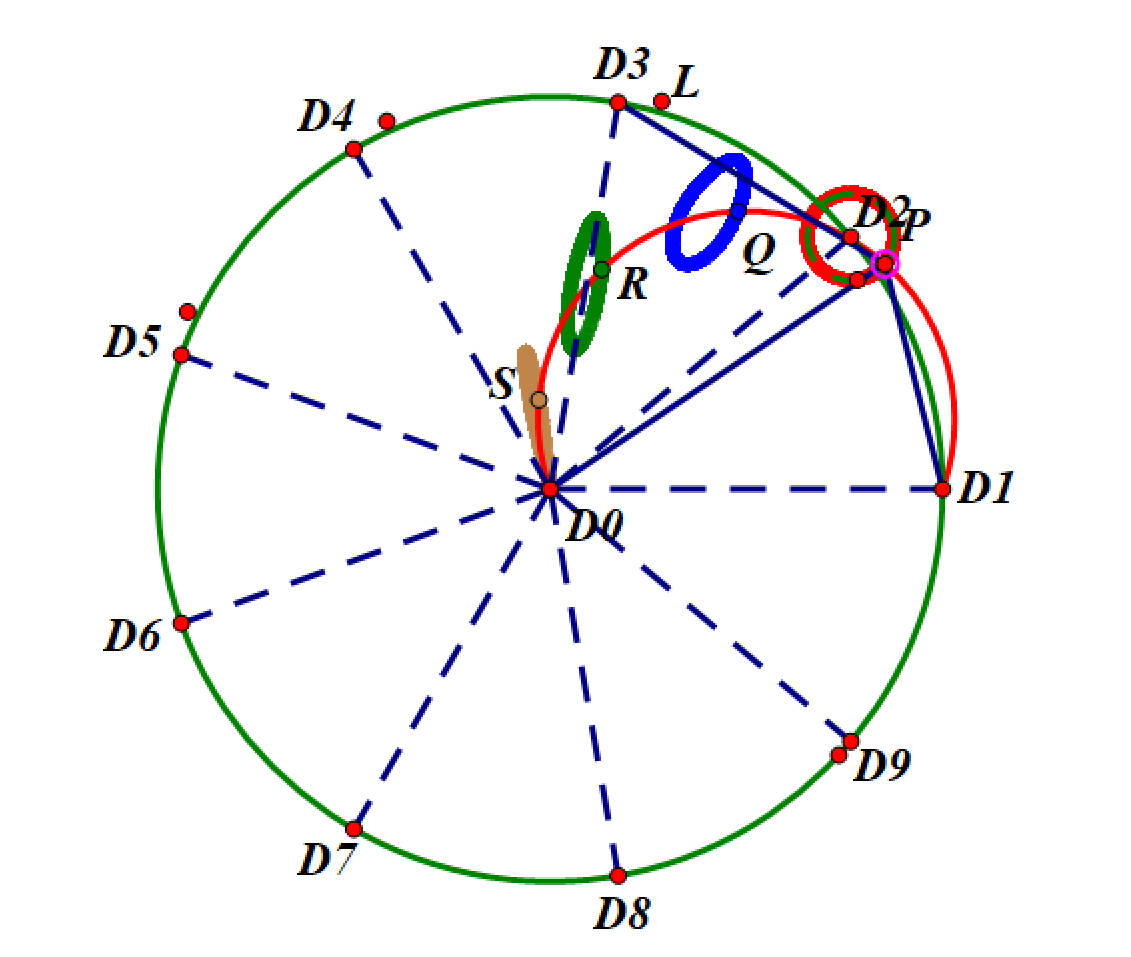
\includegraphics[width=0.43\linewidth]{../figures/7}}
				\subfloat[$r_0$处于临界时的运动轨迹情况]{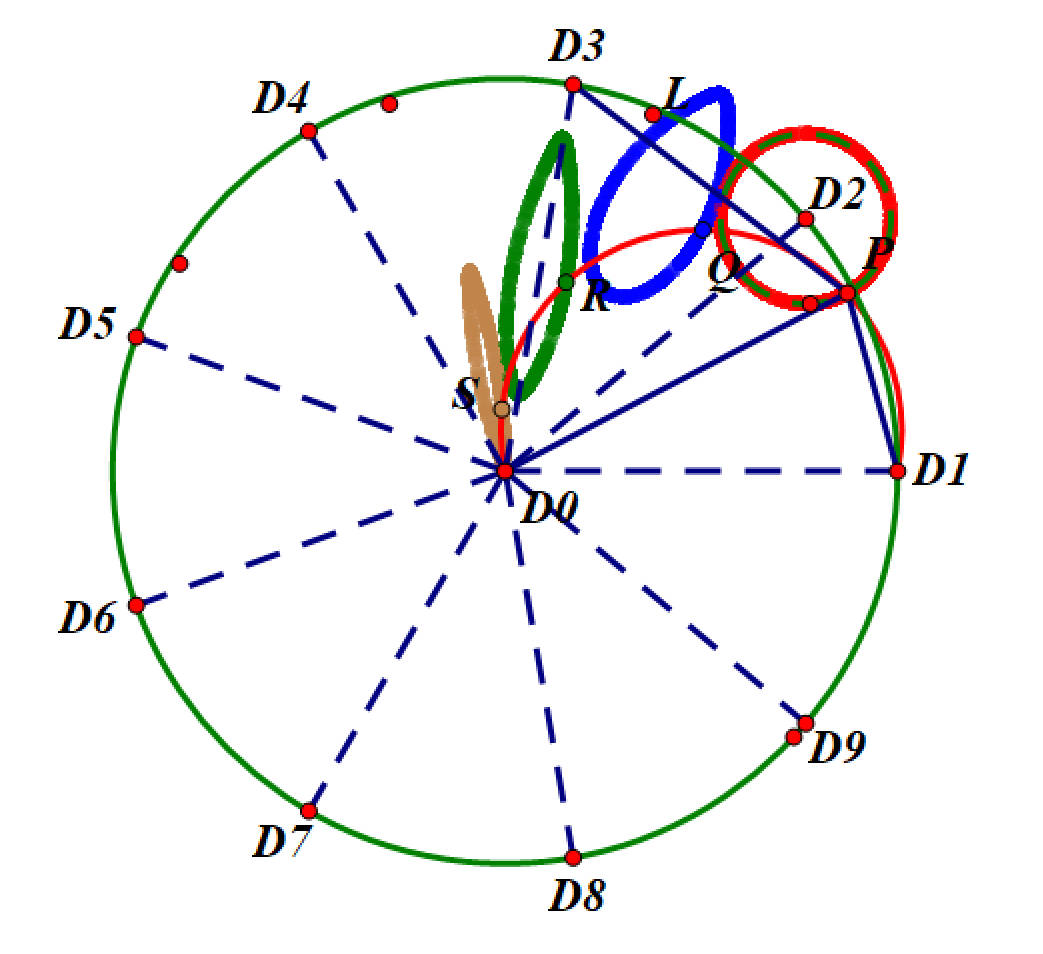
\includegraphics[width=0.4\linewidth]{../figures/8}}
				\\
				\subfloat[$r_0$很大时的运动轨迹情况]{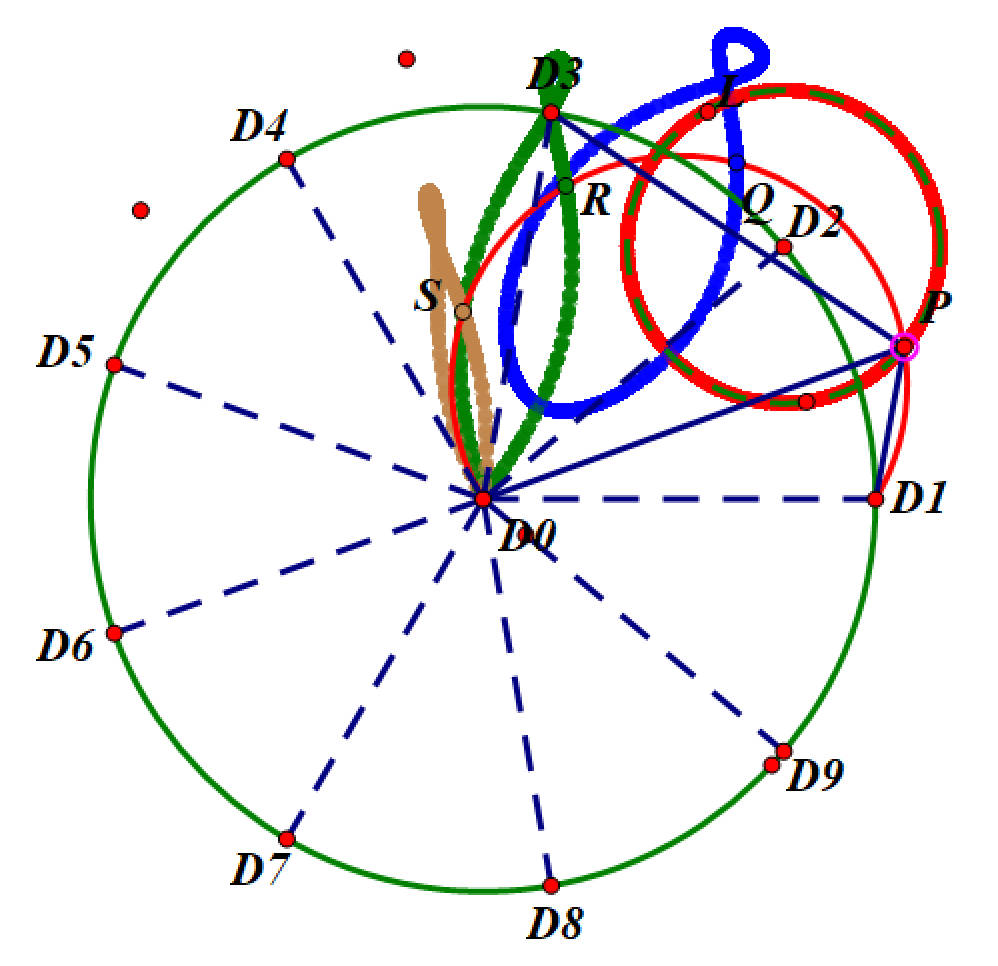
\includegraphics[width=0.4\linewidth]{../figures/9}}
				\caption{不同$r_0$的取值下$\mathcal{P}\text{(红)}\text{、}\mathcal{Q}\text{(蓝)}\text{、}\mathcal{R}\text{(绿)}\text{、}\mathcal{S}\text{(棕)}$的边界分布}
				\label{fig7}
			\end{figure}
			从图\ref{fig7}可以看出,$r_0$很大时,$\mathcal{P}\text{、}\mathcal{Q}$的边界有重叠,即$
			\exists p\in \mathcal{P},\ q\in \mathcal{Q}\ \ s.t.\ \left| \overrightarrow{pD_2} \right|\ >\left| \overrightarrow{qD_2} \right|$ 此时根据如果根据预测点到理想点最近的原则确定匿名无人机编号,将会误认为是$D_4$发射的信号,进而将自己的位置误认为$q$的位置。如图\ref{fig4}所示。
			
			我们希望存在一个最大的$r_2$,当$\lVert\omega_i\rVert \leqslant r_2$时,从正确的匿名无人机得到的解一定是所有可能解中距离理想位置最近的一个,从而使用最近点原则找到正确的发射源。
			
			使用动态几何求解器,我们求得在上述情形下$\mathcal{P}\text{、}\mathcal{Q}$边界相切时,$r_{2max}\approx 0.228\left| \overrightarrow{D_0D_1} \right|$。
			进一步,我们探索了匿名无人机变化与边界情况$r_i$的最大取值之间的关系。我们得出结论:$r_i$的最大取值与匿名无人机的的变化无关,只与待测无人机的编号i有关。
			\begin{figure}[H]
				\centering
				\subfloat[匿名无人机为$D_3$时的边界情况]{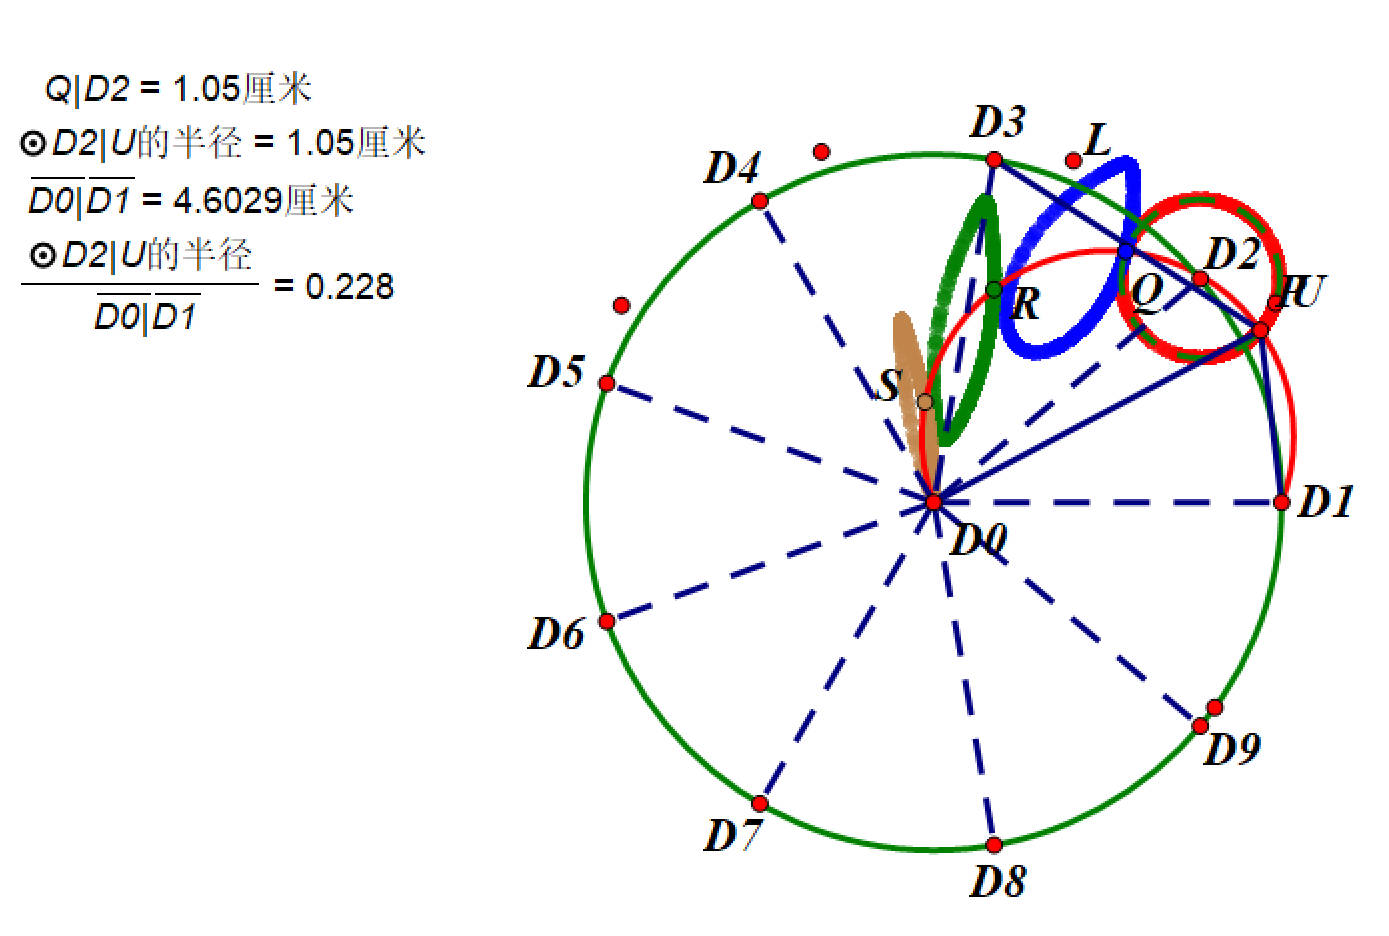
\includegraphics[width=0.45\linewidth]{../figures/10}}
				\subfloat[匿名无人机为$D_4$时的边界情况]{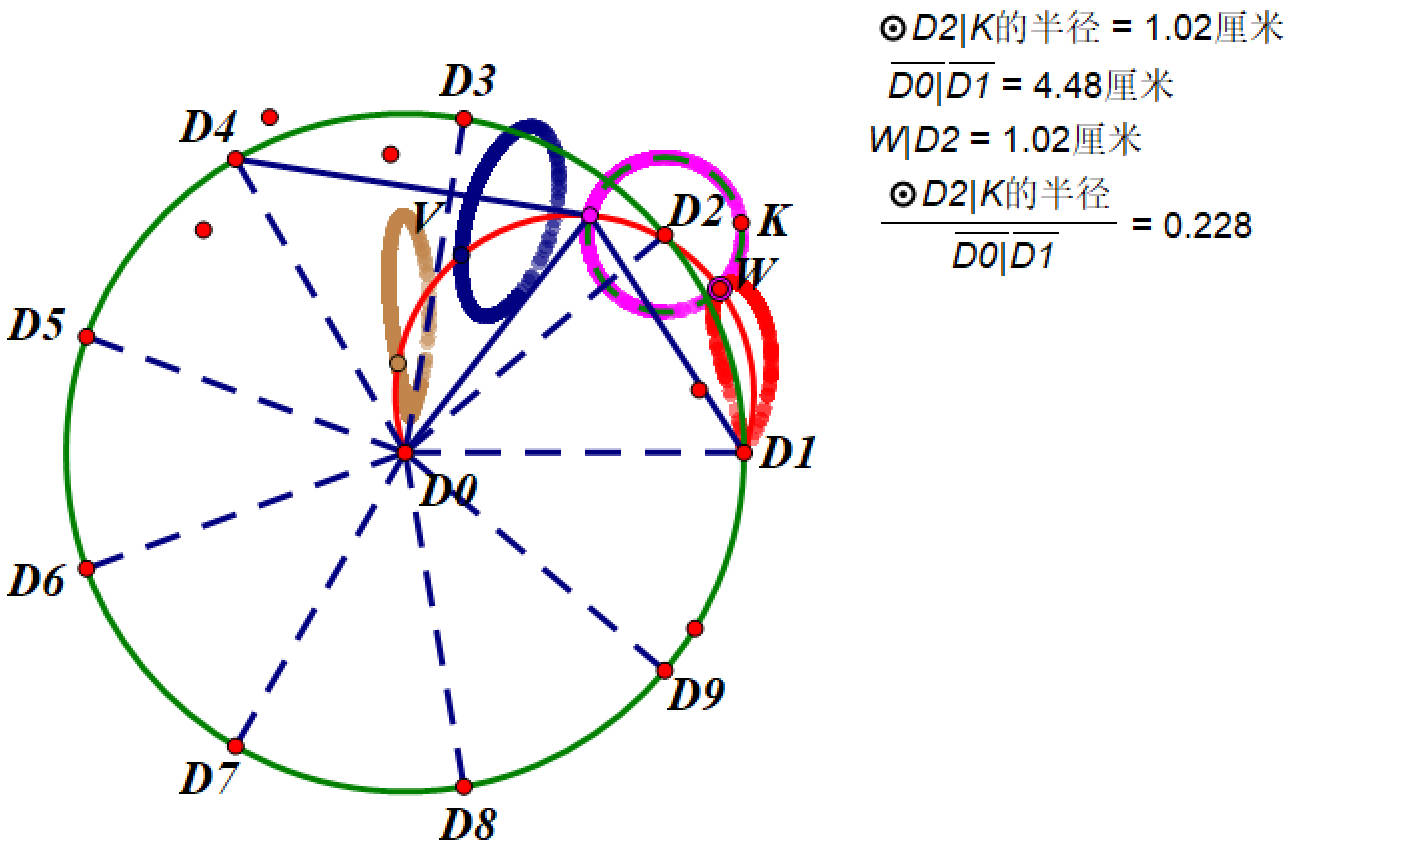
\includegraphics[width=0.45\linewidth]{../figures/11}}
				\caption{不同匿名无人机情况对于$D_2$唯一解边界情况的影响}
				\label{fig10}
			\end{figure}
		
			进一步,我们探索了不同待测无人机的最大误差范围。
			根据我们的模拟,我们有如下临界情况,见图\ref{fig12}.
			\begin{figure}[htb]
				\centering
				\subfloat[待测无人机为$D_3$时的边界情况]{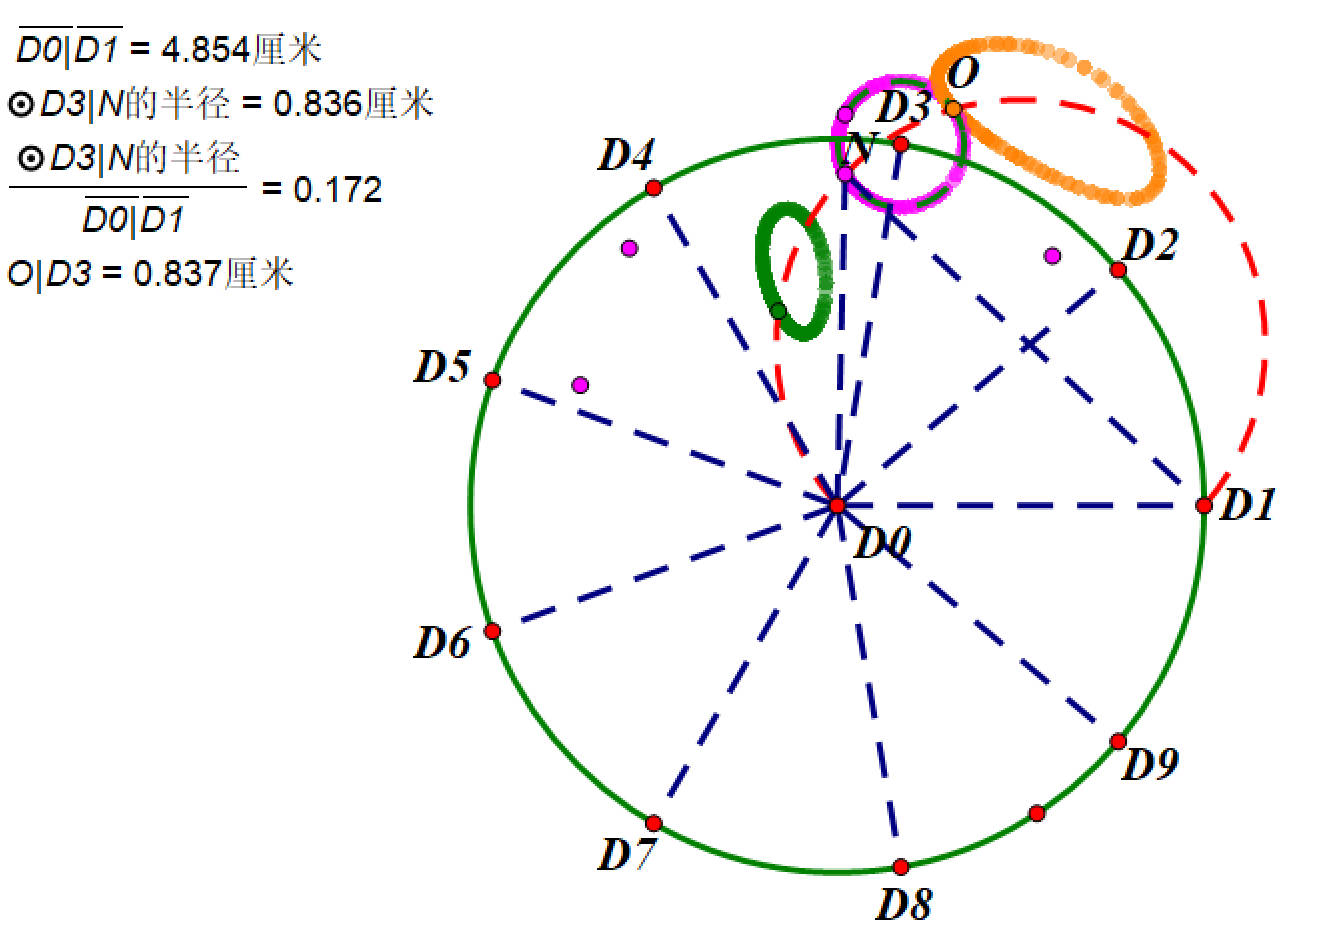
\includegraphics[width=0.5\linewidth]{../figures/12}}
				\subfloat[待测无人机为$D_4$时的边界情况]{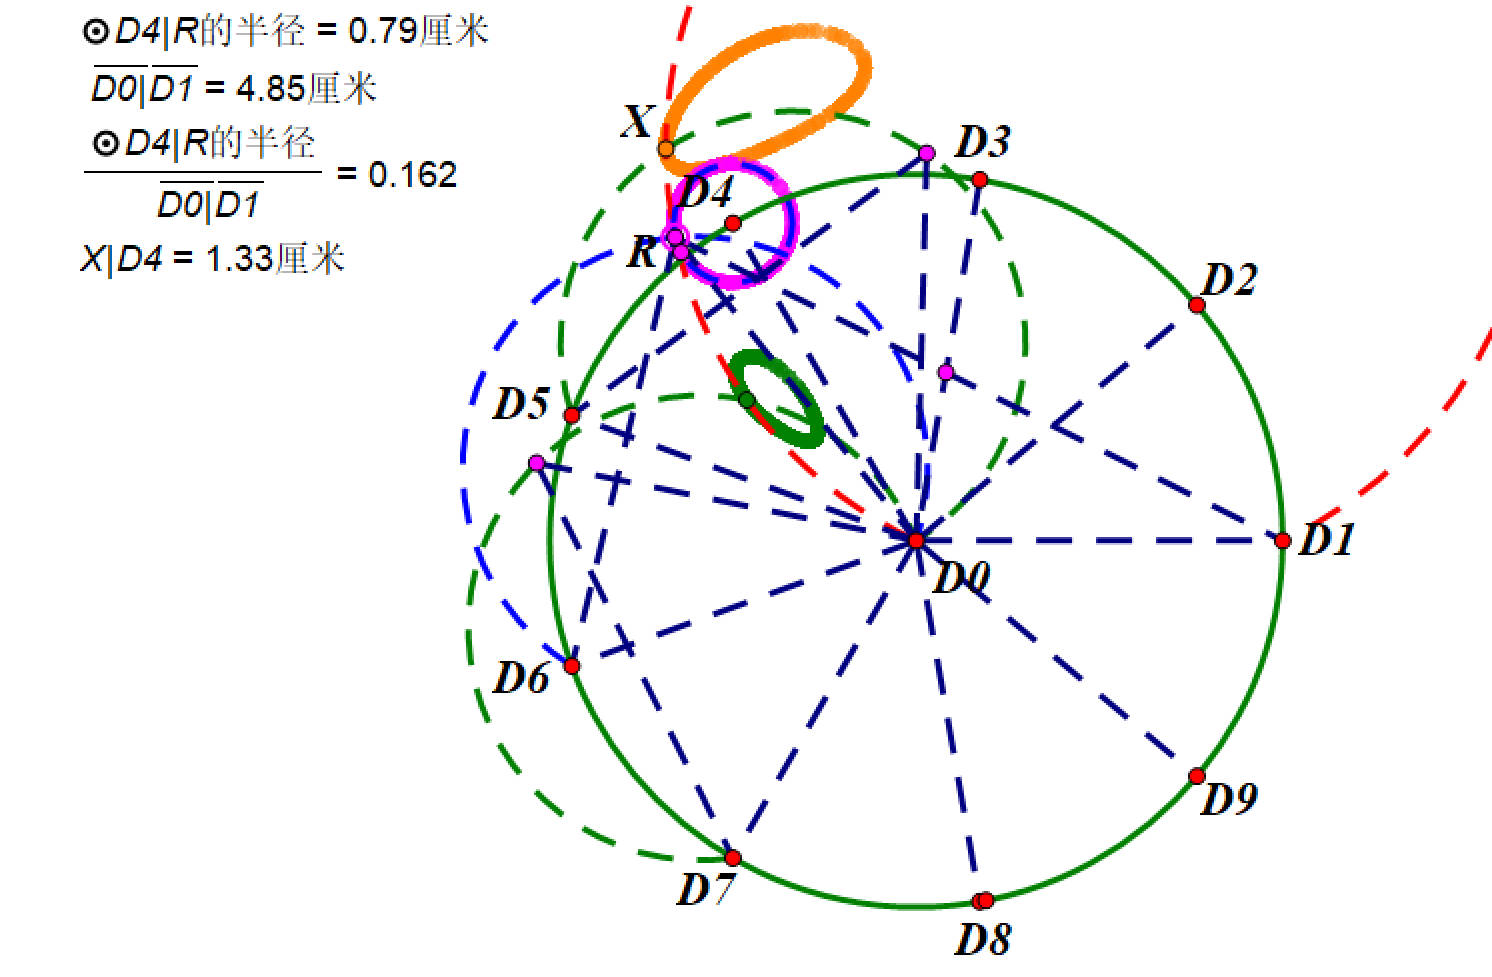
\includegraphics[width=0.5\linewidth]{../figures/13}}
				\\
				\subfloat[待测无人机为$D_5$时的边界情况]{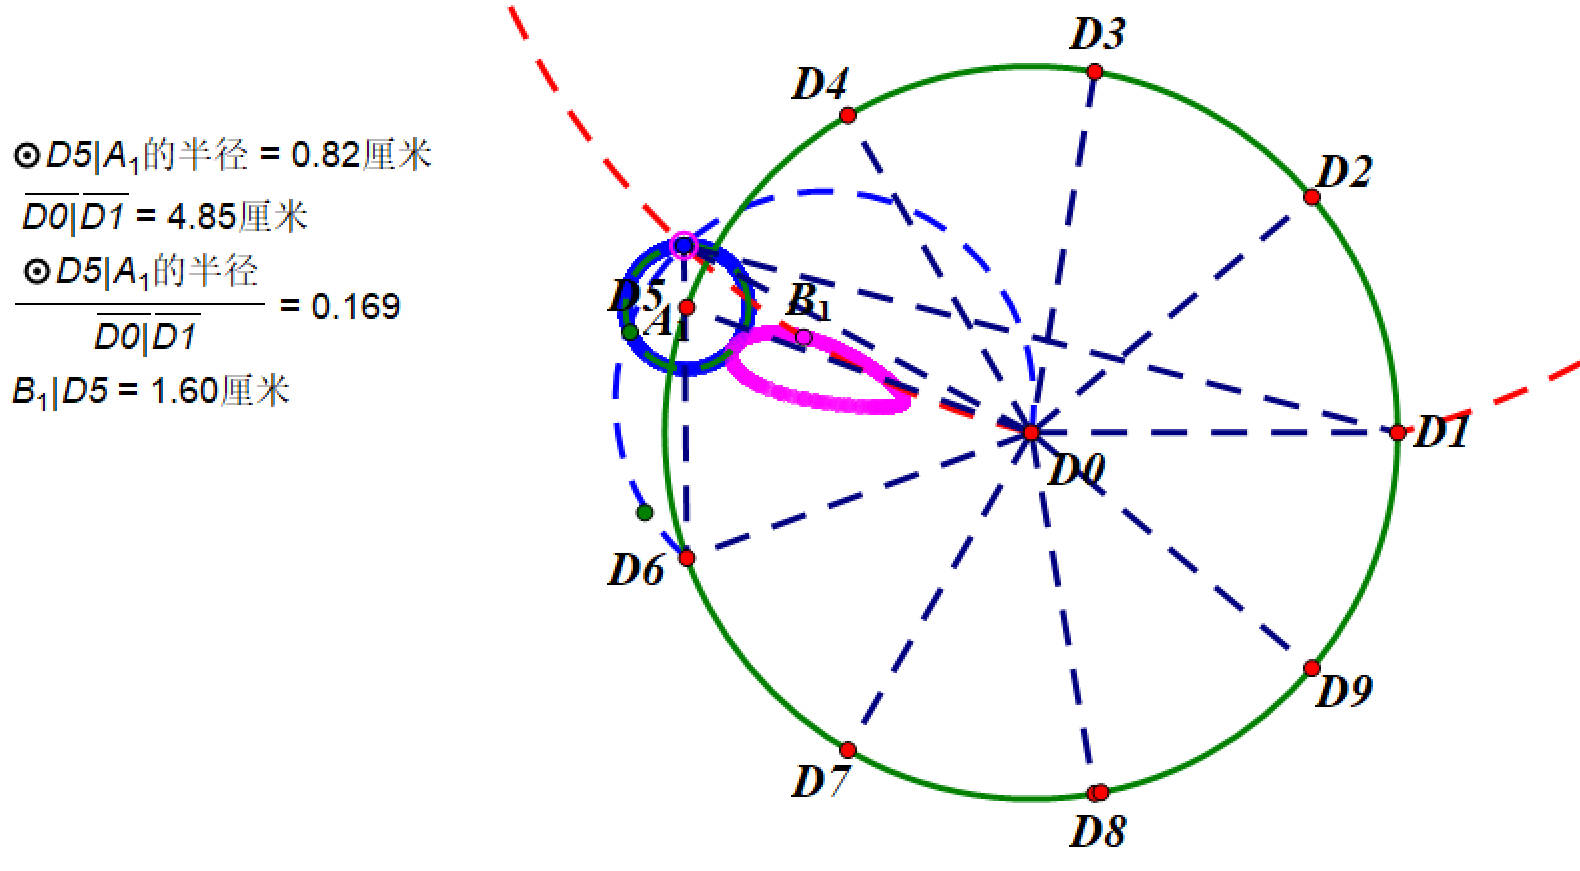
\includegraphics[width=0.5\linewidth]{../figures/14}}
				\caption{不同待测无人机唯一解边界情况}
				\label{fig12}
			\end{figure}
			\par
			令$r_i$为第i个无人机作为待测无人机时,有单一解时$\overrightarrow{\widehat{D_i}D_i}$的模长。
			我们分别得出,$r_{3max}\approx 0.172\left| \overrightarrow{D_0D_1} \right|,r_{4max}\approx 0.162\left| \overrightarrow{D_0D_1} \right|,r_{5max}\approx 0.169\left| \overrightarrow{D_0D_1} \right|$。
			根据对称性,我们同理可得$D_6,D_7,D_8,D_9$分别为待测无人机的情况。
			
			综上,我们进而给出对于任意的无人机,其“偏差较小”的数学定义为$|\overrightarrow{\widehat{D_i}D_i|}<0.162|\overrightarrow{\widehat{D_0}D_1}|$。若知道具体编号,则可以适用不同的边界情况数据。
			
			观察第三问中给出的数据,发现所有的无人机有偏位置坐标均符合我们对于“偏差较小”的定义,我们认为此定义适用于本题的所有情形。
			
			综上,在合理定义“较小偏差”后,当所有无人机的位置符合的情况下,我们即可利用上述原则确定匿名第三者,进而使用第一问中的结论就可求得待求无人机的位置。
			
			\paragraph{对于圆上两个无人机定位充要性的论证}
			本部分在开头即提出了我们的结论,即圆上两架无人机就可以确定任何一个无人机的位置。其证明将会从必要性和充分性两个方面进行说明。
			\begin{itemize}
				\item	首先在本题的题设中,圆上均匀分布着9个无人机,不存在任意两架无人机与圆心共线的问题。
				\item	必要性:从前面的论证易得,使用一架圆周上的无人机与圆心配合时,此时待测无人机只能测到一个角度,此时的解空间即为定弦与定角所确定的圆弧,不能确定无人机的位置。
				\item	充分性:在“较小偏差”的唯一解定义下,使用两架无人机进行测量,可以使用算法排除多解情况,此时位置被唯一确定,因此两架圆上无人机的定位是充分的。
			\end{itemize}
			
		\subsection{问题一(3)}
			\par 我们将问题三分为两个子问题:
			\begin{itemize}
				\item 选择发射信号飞机数量
				\item 设计无人机编队位置调整方案
			\end{itemize}
			下面分别对两个问题进行解答。
			\subsubsection{选择发射信号飞机数量}
			基于问题一,除去圆心编号为FY00的无人机外,至少还需要2架圆上的飞机,才能实现其余飞机的有效定位。在题目限制的条件下,我们可以选择的2架飞机发射信号,或选择3架飞机发射信号。通过对以下因素的分析,我们可以发现,选择3架飞机发射信号明显优于选择2架飞机发射信号:
			\begin{itemize}
				\item 定位误差
				\item 迭代次数
				\item 总电磁信号发送次数:基于电磁静默原则,总电磁信号发送次数尽可能越小越好。其值为:发射信号无人机数量$\times$迭代调整次数
			\end{itemize}
			%在本问中发射信号的无人机可能与其理想位置略有偏差,对待定位无人机的得到方%向信息带来误差。若每次选择相同的无人机来发射信号,会使误差产生累计,导致%其余无人机不仅不会收敛到理想位置,还会与理想位置的偏差越来越大。为了在一定程度上消除误差,每次随机在圆上选取planeB(planeB不为planeA),因为基于随机的方法和初始情况下,无人机在理想位置周围有一个较小的随机偏差,随机选取发射信号无人机可以使得多次迭代之间的方向信息误差相互中和。
			
			%%%%%%%%%%%%%%%%%%%%%%%%%%%%%%%%%%%%%%%%%%%%%%%%%%%%%%%%%%%%%%%%%%%%%%%%%%%%%%%
			\subsubsection{}
			\paragraph{双机定位与三机定位的误差分析}
			如图\ref{fig16}所示,我们将定位每一轮次中的定位情形作此抽象。对于发射信号的三架无人机$D_2,D_5,D_8$,有其实际位置$\widehat{D_2}\in C_2,\widehat{D_5} \in C_1,\widehat{D_8}\in C_3$,$C_1,C_2,C_3$为对应无人机的“微小偏差”区域(比例有所夸张),同时有待定位的无人机$\widehat{D_3}$,此时待定位无人机共能测得三个夹角$\angle \widehat{D_5}\widehat{D_3}D_0$,$\angle D_0\widehat{D_3}\widehat{D_8}$,$\angle \widehat{D_8}\widehat{D_3}\widehat{D_2}$。此时选取其中两个无人机就可以使用上述方法确定D的坐标,此时的三个测量值记为$D_{30},D_{31},D_{32}$。在双机定位的情况下若测量结果为$D_{30}$,此时的误差就是$|\overrightarrow{\widehat{D_3}D_{30}}|$,而在三机定位的情况下,存在一定概率使$\overrightarrow{\widehat{D_3}D_{30}}+\overrightarrow{\widehat{D_3}D_{31}}+\overrightarrow{\widehat{D_3}D_{32}} < min\{\overrightarrow{\widehat{D_3}D_{30}},\overrightarrow{\widehat{D_3}D_{31}},\overrightarrow{\widehat{D_3}D_{33}}\}$从而降低误差。
			\begin{figure}[H]
				\centering
				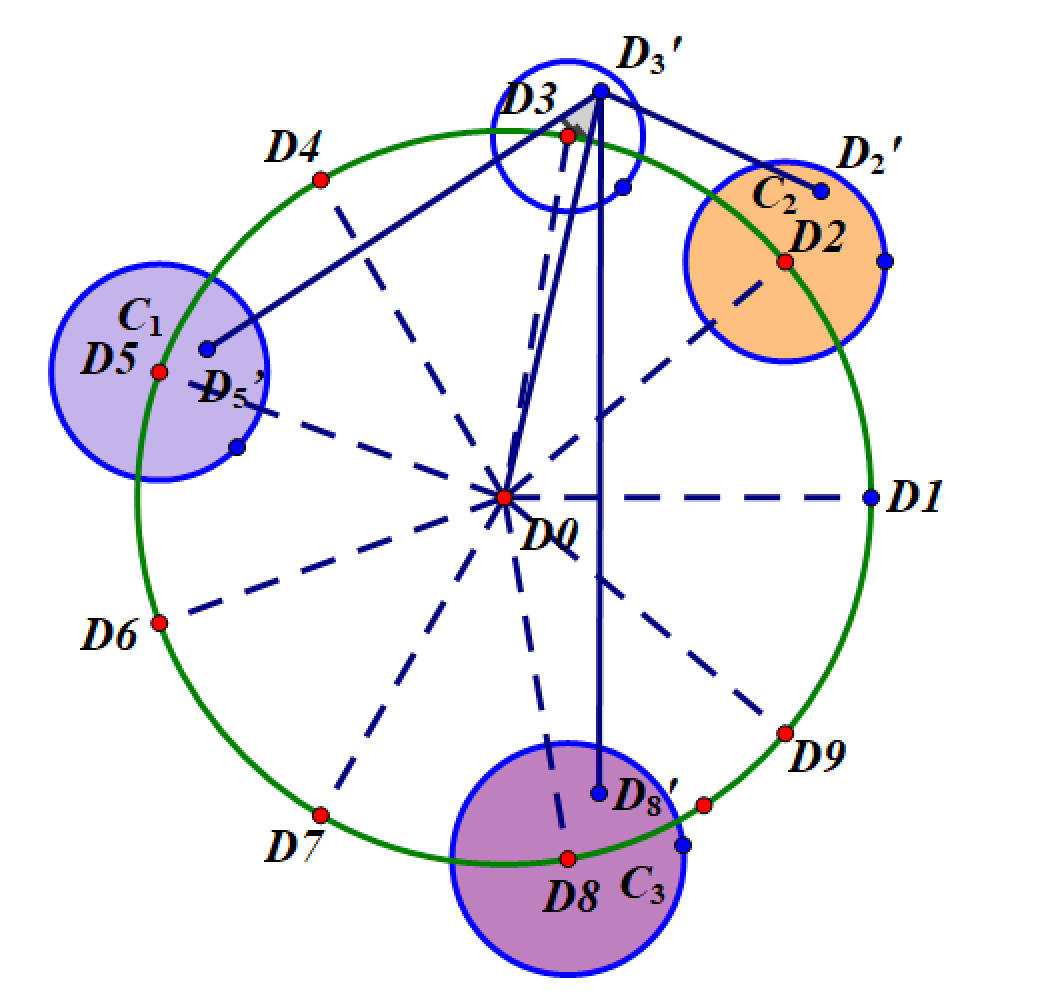
\includegraphics[width=0.5\linewidth]{./figures/16}
				\caption{定位问题的数学抽象}
				\label{fig16}
			\end{figure}
			不可否认的是,在此种情况下,亦存在$\overrightarrow{\widehat{D_3}D_{30}}+\overrightarrow{\widehat{D_3}D_{31}}+\overrightarrow{\widehat{D_3}D_{32}} > min\{\overrightarrow{\widehat{D_3}D_{30}},\overrightarrow{\widehat{D_3}D_{31}},\overrightarrow{\widehat{D_3}D_{33}}\}$的情况,为了验证本方法是否可行,对于使用计算机对于随机情况进行统计分析。
			\begin{figure}[H]
				\centering
				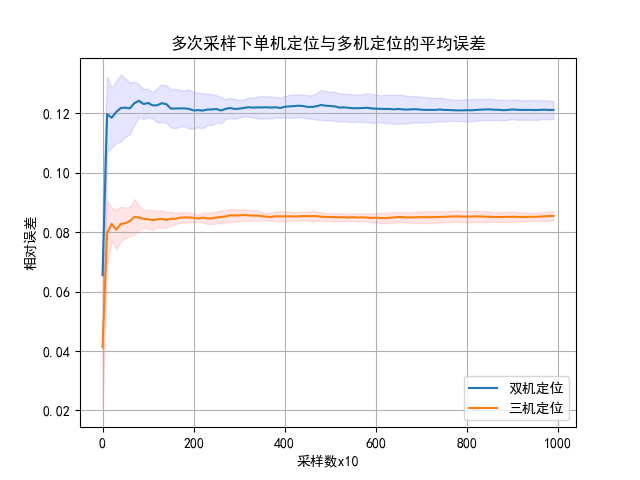
\includegraphics[width=0.75\linewidth]{./figures/15}
				\caption{多次采样下双机与三机系统的平均误差}
				\label{fig15}
			\end{figure}
			经过1000次随机采样,使用双机与三机系统对圆上每个点进行位置计算的平均误差如图\ref{fig15}所示。经统计分析,在双机系统进行位置计算时,平均误差约为$0.12R$,而使用多机系统时,平均误差降至$0.086R$,有$28.3\%$的性能提升。
			
			\paragraph{对于一种特殊情况的讨论}
			在建模的过程中,我们意识到了一种特殊情况如图\ref{fig17},此时所有圆上的无人机都均匀分布或近似均匀分布在圆上,但圆心$D_0$偏移到了$\widehat{D_0}$的位置,此时也可以使用上述方法进行调整,使新圆的圆心为$\widehat{D_0}$。然而,此时最有的调整方案应该是移动圆心的位置使其回到$D_0$,但是考虑到本题需要在每次令中心无人机发射信号,\textbf{其余}无人机接收信号,中心无人机不能获取自身的位置信息,所以调整圆心的方案不可行。
			\begin{figure}[H]
				\centering
				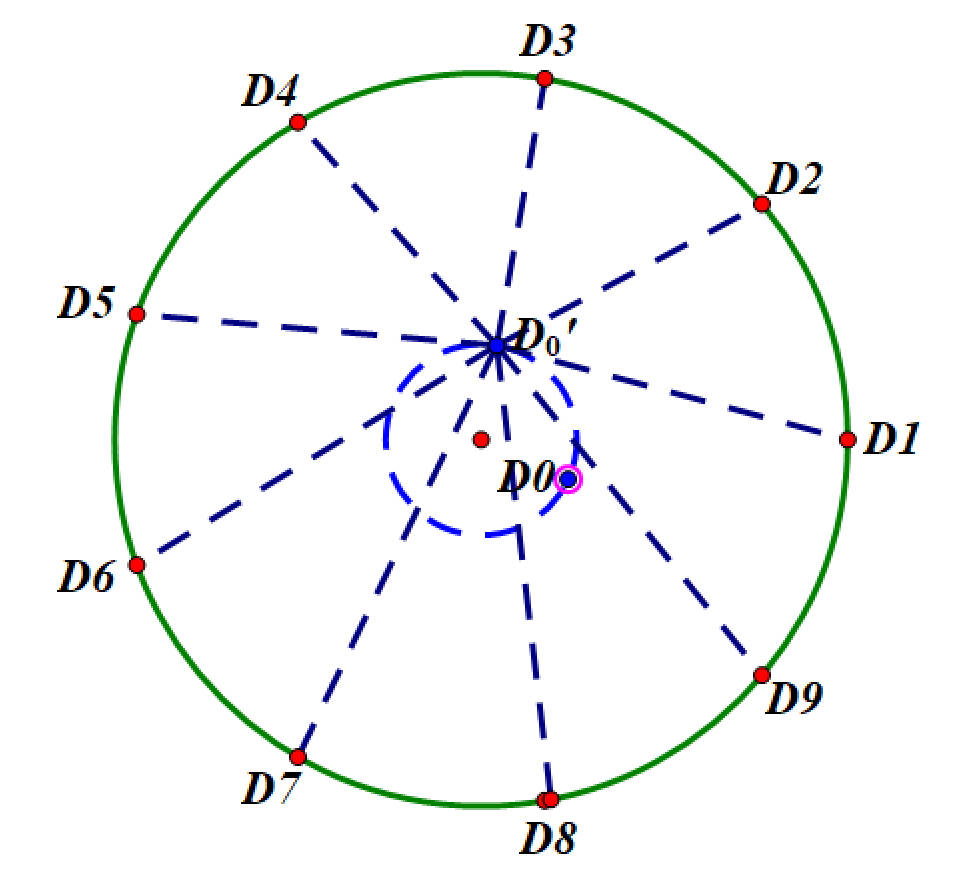
\includegraphics[width=0.45\linewidth]{./figures/17}
				\caption{圆心偏移的特殊情况}
				\label{fig17}
			\end{figure}
			
			
			
			%%%%%%%%%%%%%%%%%%%%%%%%%%%%%%差两种选择的分析%%%%%%%%%%%%%%%%%%%%%%%%%%%%%
			
			
			\subsubsection{无人机编队位置调整方案}
			我们定义一次迭代过程为:1.选择3架无人机与编号为FY00的无人机一起发射信号,2.其余无人机接收信号并定位位置,3.其余无人机进行位置调整。从初始情况开始,通过多次迭代,将机群调整为理想分布。
			\paragraph{选择发射信号无人机}
			根据5.3.1节的分析,我们每次选择理想位置将圆三等分的三架无人机发射信号,采用轮流的方式,第1次采用FY01、FY04、FY07,第2次采用FY02、FY05、FY08,第3次采用FY03、FY06、FY09...进行发射信号。
			\begin{figure}[htb]
				\centering
				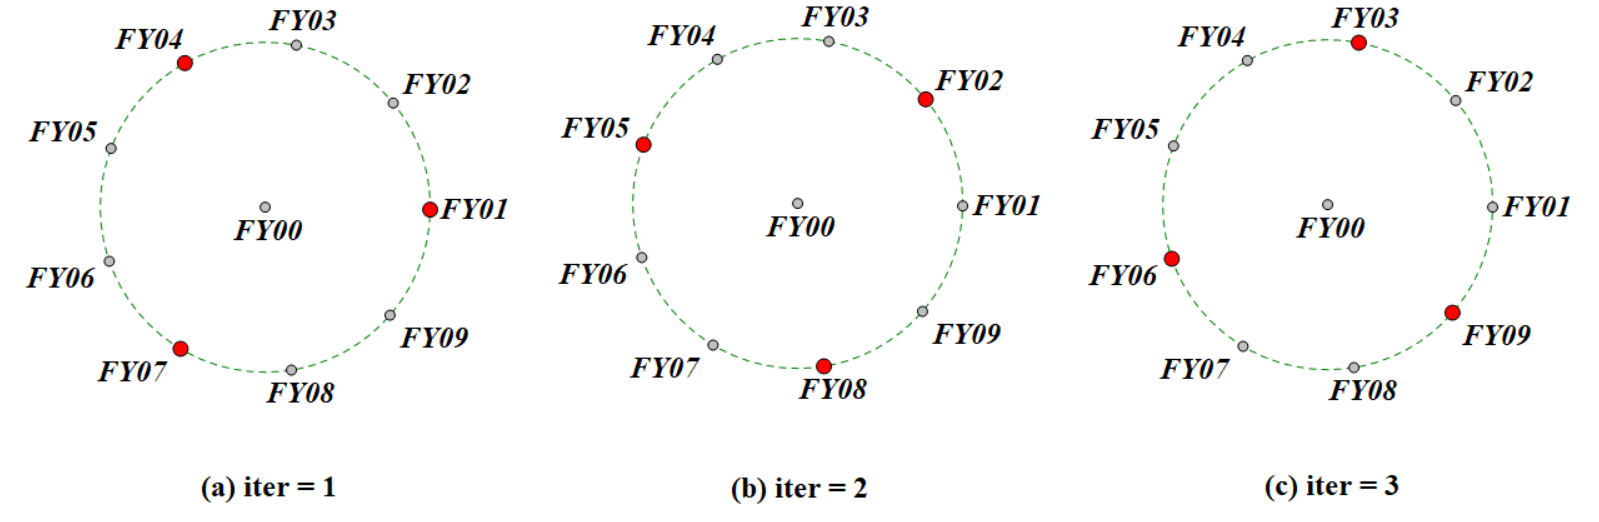
\includegraphics[width=1.0\linewidth]{./figures/发射信号无人机示意图}
				\caption{发射信号无人机选择示意图(图示位置为理想位置)}
				\label{发射信号飞机}
			\end{figure}
			\paragraph{无人机定位}
			对圆上无人机,出去发射信号的无人机,识别出接收信号的来源,该问题变成了利用编号FY00无人机与圆上3架确定编号的无人机进行定位的问题。记定位得到测量位置$(x_{measure},y_{measure})$,根据问题一,取其中2个发射信号可以得到定位,共有$C^2_3=3$种结果,如下所示:
			$$(x_{measure}^1,y_{measure}^1),(x_{measure}^2,y_{measure}^2),(x_{measure}^3,y_{measure}^3)$$
			对3个测量位置取平均,得到结果飞机的位置估计$(\hat{x},\hat{y})$:
			$$
			\left\{ \begin{array}{l}  \hat{x}=\sum_{i=1}^3{x_{measure}^{i}}\\  \hat{y}=\sum_{i=1}^3{y_{measure}^{i}}\\ \end{array} \right.  
			$$
			
			\paragraph{无人机位置调整}
			定义偏差$w$为无人机理想位置与估计位置的偏差:$\boldsymbol{w}=(x_{ideal},y_{ideal}) - (\hat{x},\hat{y})$,设置参数$\eta{}$,以$\boldsymbol{w}$作为位移调整位置,调整后的位置$(x_{new},y_{new})$为:$(x_{new},y_{new})= (x_{actual},y_{actual}) - \eta{} * \boldsymbol{w}$。
			\par 调整结果如下图\ref{Polar}所示,可以看到调整后的各个无人机较为均匀的分布在统一圆周上:
			\begin{figure}[htb]
				\centering
				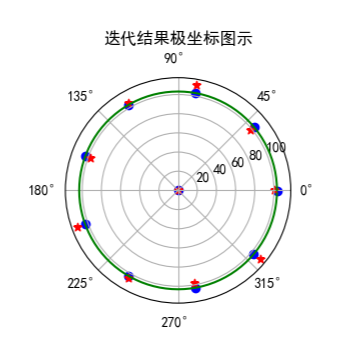
\includegraphics[width=0.7\linewidth]{./figures/Polar Axis}
				\caption{迭代调整后的结果对比图}
				\label{Polar}
			\end{figure}
			\paragraph{调整方案伪代码}
			调整方案的伪代码如下所示:
			\par
			\begin{algorithm}[H]
				\caption{无人机迭代调整算法}
				\KwIn{无人机的初始位置信息$UAV_{initial}$, 被动接受的方位信号$\alpha_1\text{与}\alpha_2$ }
				\KwOut{调整完成的最终位置信息$UAV_{hat}$}
				初始化算法的超参数:最大迭代次数$ maxIter $、学习率$ \eta $、迭代权重系数$ weight $;
				\par \For{$iter=start;iter \le maxIter;iter++$}
				{
					\#选择三架分布均匀的无人机作为一组承担发射信号的任务。
					\par  $ launch[i] =(launch[i-1] + 3) \% 9 $
					\par \For{$ i in range(1,10) 且 i ≠ launch[i] $ }
					{
						计算三架无人机中任意两架与待定位无人机的夹角 $\alpha[i],i=1,2,3 $ \;
						进而转化为第一问的情况可以计算三组测量坐标
						\par $ Compute\quad the\quad position\_measure\_list $
						\par \#将测量坐标求取均值以获得一组最终估计坐标
						\par  $ position\_estimate= Mean(position\_measure\_list) $
						\par \#计算估计坐标与理想坐标的误差
						\par$  error = ideal\_xy -position\_estimate $
						\par \#利用计算所得误差进行位置坐标的更新
						\par \If{$position\_estimate[i] < 0 or > 0 $}
						{
							\# 通过估计坐标的$ x,y $坐标的正负判断所在象限
							\par replace $position\_estimate$ with $ PolarAxisPosition $;
						}
					}
					\# 绘制初始极坐标和调整后极坐标示意图;		
				}
				\textbf{Return:}返回迭代后的无人机的 $postion$;
				\label{code}
			\end{algorithm}
		\subsection{问题二}
	\section{总结}
	
	\begin{thebibliography}{9}%宽度9
		\bibitem{bib:one} ....
	\end{thebibliography}
	\begin{appendices}
		附录的内容。
	\end{appendices}
\end{document}